\documentclass[11pt,a4paper]{article}
\usepackage[utf8]{inputenc}
\usepackage[T1]{fontenc}
\usepackage[a4paper,margin=2.5cm]{geometry}
\renewcommand{\figurename}{Figura}
\renewcommand{\tablename}{Tabela}
\usepackage{graphicx}
\usepackage{array}
\usepackage{booktabs}
\usepackage{float}
\usepackage{helvet}
\renewcommand{\familydefault}{\sfdefault}
\linespread{1.25}
\setlength{\parindent}{0pt}
\setlength{\parskip}{6pt}
\renewcommand{\thesection}{\arabic{section}.}

\begin{document}

% ===================== CABEÇALHO INSTITUCIONAL =====================
\begin{table}[H]
\centering
\renewcommand{\arraystretch}{1.4}
\begin{tabular}{|m{3.0cm}|m{3.6cm}|m{6.6cm}|}
\hline
\centering\textbf{INSTITUTO} & Curso & SI \\ \cline{2-3}
\centering\textbf{FEDERAL} & Período/Semestre & 7º Período / 2026-1 \\ \cline{2-3}
\centering\textbf{Goiano} & Disciplina & Temática em Mineração de Dados \\ \cline{2-3}
\centering\textbf{Campus} & Nome & Arthur Faria Estrela, Ricardo Issa de Sousa, Sávio Issa de Sousa \\ \cline{2-3}
\centering\textbf{Urutaí} & Data & 13 / 03 / 2026 \\ \hline
\end{tabular}
\end{table}

\vspace{0.6cm}
\begin{center}
{\Large \textbf{Relatório Técnico:}}\\[0.3cm]
{\large \textbf{Base Cheese --- Segmentação Sensorial de Queijos}}\\[0.2cm]
{\normalsize \textit{(Aprendizado Não-Supervisionado --- Clusterização K-Means)}}
\end{center}
\vspace{0.4cm}

% ===================== 1. OBJETIVO =====================
\section{Objetivo do Projeto}

Diferentemente das demais bases trabalhadas na disciplina --- todas voltadas a problemas de classificação supervisionada com uma variável-alvo definida --- a base \textit{Cheese} não possui rótulo a ser previsto. O objetivo deste estudo é, portanto, de natureza \textbf{exploratória e não-supervisionada}: descobrir \textbf{agrupamentos naturais (clusters)} de queijos a partir de suas características sensoriais, identificando perfis de produto que não estão explicitamente codificados nos dados. A meta técnica foi segmentar as amostras em grupos internamente homogêneos e externamente heterogêneos, e, sobretudo, \textbf{traduzir cada cluster em conhecimento interpretável} sobre o perfil sensorial que o define (aroma, aparência, textura e sabor).

% ===================== 2. LIMPEZA =====================
\section{Tratamento e Limpeza de Dados (Data Cleaning)}

A base é composta por \textbf{240 avaliações sensoriais} originalmente distribuídas em 29 colunas, resultantes de painéis de degustação em que provadores treinados pontuam diferentes atributos de cada queijo. As variáveis seguem uma convenção de prefixos que organiza os descritores em blocos: \textbf{N.} (aroma/odor --- \textit{nose}), \textbf{E.} (aparência e textura visual --- \textit{exterior}), \textbf{H.} (resistência/dureza) e \textbf{M.} (sensações em boca --- \textit{mouth}: cremosidade, firmeza, derretimento, salgado, ácido, doce, etc.).

A seleção isolou os \textbf{28 atributos numéricos} associados a esses descritores. Em seguida, garantiu-se a tipagem numérica correta de todas as colunas (conversão explícita), descartaram-se variáveis com excesso de valores ausentes (limiar de 50\%) e removeram-se os registros remanescentes com dados faltantes. Após essa etapa de saneamento, o conjunto manteve sua volumetria integral de 240 observações válidas, preservando toda a amostra para a análise.

% ===================== 3. PRÉ-PROCESSAMENTO =====================
\section{Pré-processamento e Padronização}

O algoritmo K-Means baseia-se em \textbf{distâncias euclidianas} para alocar observações aos centróides. Por consequência, variáveis medidas em magnitudes diferentes distorceriam o cálculo, fazendo com que atributos de maior amplitude dominassem artificialmente o agrupamento. Para neutralizar esse efeito, todas as variáveis sensoriais foram submetidas à \textbf{padronização Z-score} (centralização na média e escalonamento pelo desvio-padrão, função \texttt{scale}). Esse passo, frequentemente negligenciado em análises rudimentares, é \textbf{condição indispensável} para que cada descritor sensorial contribua de forma equânime para a definição dos grupos, e foi tratado aqui como etapa obrigatória do pipeline.

% ===================== 4. NÚMERO DE CLUSTERS =====================
\section{Determinação do Número de Clusters (Método do Cotovelo)}

Uma das decisões mais críticas --- e mais frequentemente arbitrárias --- em clusterização é a escolha do número de grupos \textit{k}. Em vez de fixar esse valor por conveniência, recorreu-se ao \textbf{Método do Cotovelo (\textit{Elbow Method})}, que avalia a \textbf{soma dos quadrados intra-cluster (WSS)} para uma faixa crescente de valores de \textit{k}. A curva resultante decresce rapidamente até o ponto em que adicionar novos clusters deixa de reduzir significativamente a variância interna --- o "cotovelo". A inspeção do gráfico (Figura 1) fundamentou matematicamente a escolha de \textbf{k = 3}, ponto a partir do qual os ganhos de homogeneidade tornam-se marginais, equilibrando ajuste e parcimônia.

% ===================== 5. MODELAGEM =====================
\section{Modelagem: Algoritmo K-Means}

A segmentação final foi obtida com o algoritmo \textbf{K-Means} configurado com \textit{k} = 3. Para mitigar a sensibilidade do método à inicialização aleatória dos centróides --- que pode aprisioná-lo em mínimos locais sub-ótimos --- empregou-se o parâmetro \texttt{nstart = 25}, que executa 25 inicializações independentes e retém a partição de menor variância intra-cluster. Uma semente fixa (\texttt{set.seed(123)}) garantiu a \textbf{reprodutibilidade} integral do experimento.

O agrupamento resultante distribuiu as 240 amostras de forma notavelmente equilibrada entre os três grupos:

\begin{table}[H]
\centering
\renewcommand{\arraystretch}{1.3}
\begin{tabular}{ccc}
\toprule
\textbf{Cluster} & \textbf{Nº de amostras} & \textbf{Participação} \\
\midrule
Cluster 1 & 84 & 35,0\% \\
Cluster 2 & 75 & 31,2\% \\
Cluster 3 & 81 & 33,8\% \\
\midrule
\textbf{Total} & \textbf{240} & \textbf{100\%} \\
\bottomrule
\end{tabular}
\end{table}

% ===================== 6. AVALIAÇÃO E CONCLUSÃO =====================
\section{Avaliação dos Resultados e Conclusão Técnica}

A qualidade da partição foi avaliada pela decomposição da variância total. A razão entre a \textbf{soma de quadrados entre clusters} e a soma total atingiu \textbf{19,6\%} (\textit{between/total SS}), valor coerente para dados sensoriais reais, em que as fronteiras entre perfis são naturalmente difusas --- não há, afinal, rótulos rígidos separando os queijos. Para interpretar e visualizar os grupos, aplicou-se a \textbf{Análise de Componentes Principais (PCA)}: as duas primeiras componentes concentraram \textbf{29,9\%} da variância total (PC1 = 16,8\%; PC2 = 13,1\%), o suficiente para evidenciar a separação dos clusters no plano (Figura 2) e identificar, via contribuição das variáveis (Figura 3), quais atributos sensoriais mais estruturam essa separação.

O verdadeiro valor da análise, contudo, está na \textbf{leitura do perfil médio de cada cluster} (Figura 4), que permitiu rotular os grupos em três identidades sensoriais nítidas:

\textbf{Cluster 1 --- "Cremoso e Amanteigado":} caracteriza-se por elevada cremosidade (\textit{M.Creaminess} = 8,3), forte capacidade de derretimento (\textit{M.Melt.down} = 9,4), brilho acentuado (\textit{E.Shiny} = 9,8), notas amanteigadas (\textit{M.Butter} = 9,6) e salgadas (\textit{M.Salt} = 7,4), aliados a baixa firmeza (\textit{M.Firm} = 5,0). Representa o queijo macio, untuoso e que se desfaz na boca.

\textbf{Cluster 2 --- "Ácido e Magro":} marcado pela acidez dominante (\textit{M.Sour} = 8,6) e textura arenosa/calcária (\textit{M.Chalky} = 6,1), com baixos índices de gordura (\textit{M.Fat} = 6,2), manteiga (\textit{M.Butter} = 5,8) e sal (\textit{M.Salt} = 4,8). Corresponde ao perfil mais leve, azedo e seco.

\textbf{Cluster 3 --- "Firme e Gorduroso":} definido pela alta firmeza (\textit{M.Firm} = 9,4), resistência à mordida (\textit{M.Resistance} = 8,5; \textit{H.Resistance} = 8,7) e elevado teor gorduroso (\textit{M.Fat} = 9,5), com baixo derretimento (\textit{M.Melt.down} = 6,2) e aparência opaca (\textit{E.Shiny} = 6,4). É o queijo denso, encorpado e estruturado.

\textbf{Conclusão técnica:} o estudo demonstra que, mesmo sem nenhuma variável-alvo, é possível extrair estrutura e significado de dados sensoriais. O K-Means, sustentado por padronização rigorosa e por uma escolha de \textit{k} matematicamente justificada, não apenas separou as amostras em grupos equilibrados, mas revelou \textbf{três perfis de queijo industrialmente acionáveis} --- cremoso, ácido-magro e firme-gorduroso. Mais do que rodar o algoritmo, o diferencial metodológico foi \textbf{transformar centróides abstratos em conhecimento de produto interpretável}, evidenciando domínio do paradigma não-supervisionado da Mineração de Dados.

% ===================== 7. ANÁLISE VISUAL =====================
\section{Análise Visual dos Resultados}

A materialização gráfica consolida os achados numéricos. O \textbf{gráfico do cotovelo} (Figura 1) fundamenta a escolha de três grupos; o \textbf{mapa de clusters sobre as componentes principais} (Figura 2) confirma visualmente a separação das três nuvens de pontos; o \textbf{círculo de correlação das variáveis} (Figura 3) revela quais descritores puxam cada eixo --- opondo, por exemplo, cremosidade/derretimento a firmeza/resistência; e o \textbf{heatmap de perfis} (Figura 4) sintetiza, em uma única imagem, a assinatura sensorial de cada cluster, validando os rótulos atribuídos.

% ===================== 8. GRÁFICOS =====================
\section{Gráficos}

\begin{figure}[H]
\centering
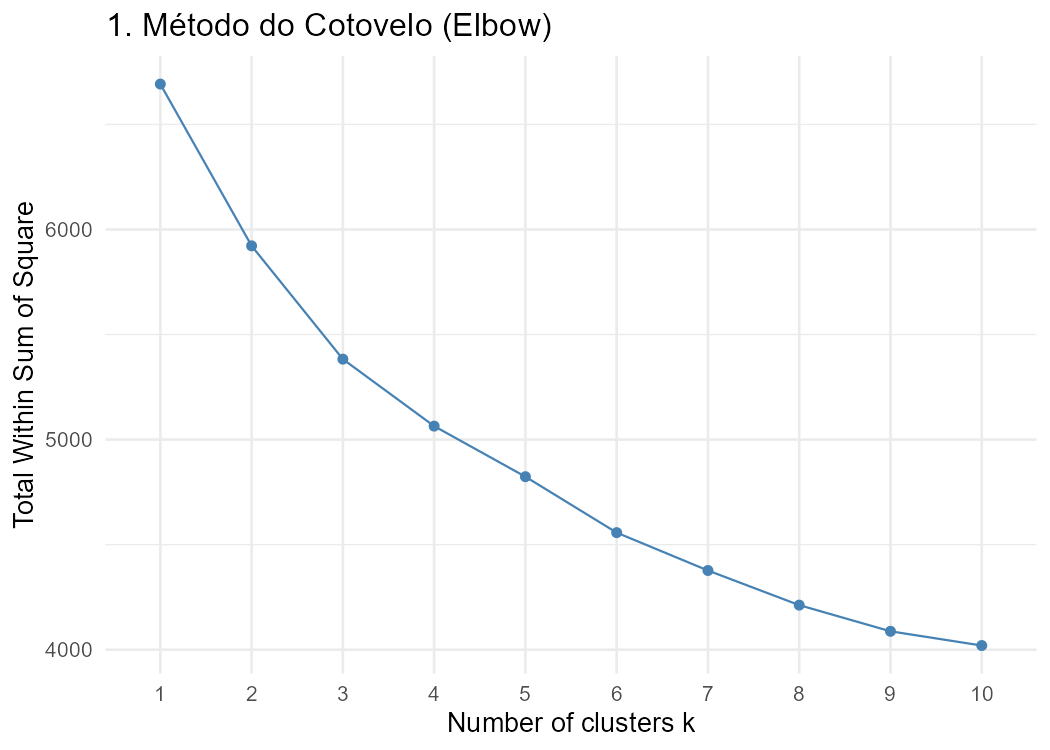
\includegraphics[width=0.80\textwidth]{fig/01_cotovelo.png}
\caption{Método do Cotovelo --- soma de quadrados intra-cluster (WSS) por número de grupos. O "cotovelo" fundamenta a escolha de k = 3.}
\end{figure}

\begin{figure}[H]
\centering
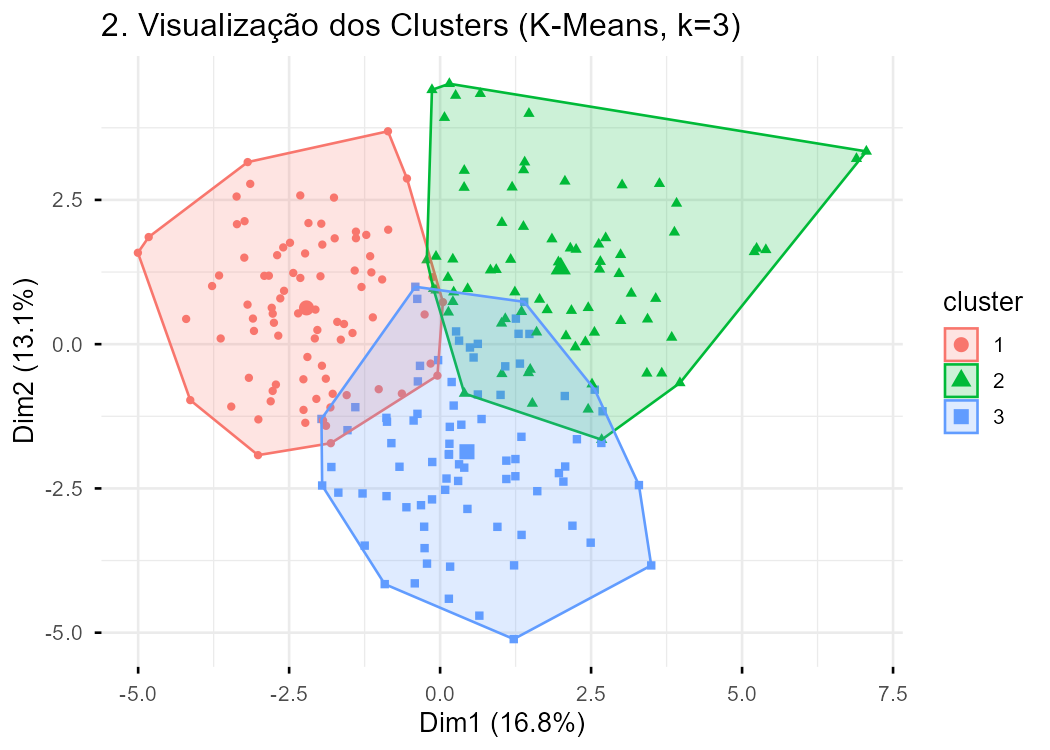
\includegraphics[width=0.80\textwidth]{fig/02_clusters.png}
\caption{Visualização dos três clusters projetados sobre as duas primeiras componentes principais (PC1 = 16,8\%; PC2 = 13,1\%).}
\end{figure}

\begin{figure}[H]
\centering
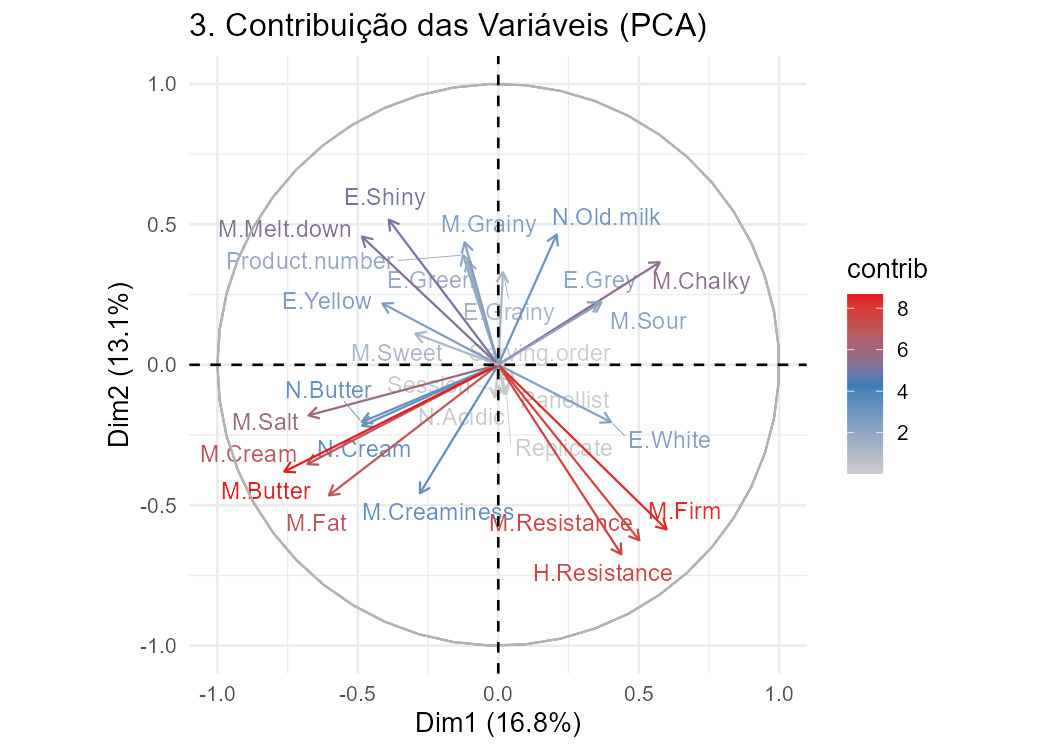
\includegraphics[width=0.80\textwidth]{fig/03_pca_var.png}
\caption{Contribuição das variáveis sensoriais nas componentes principais. Quanto mais intensa a cor e mais longo o vetor, maior a influência do atributo na estrutura dos dados.}
\end{figure}

\begin{figure}[H]
\centering
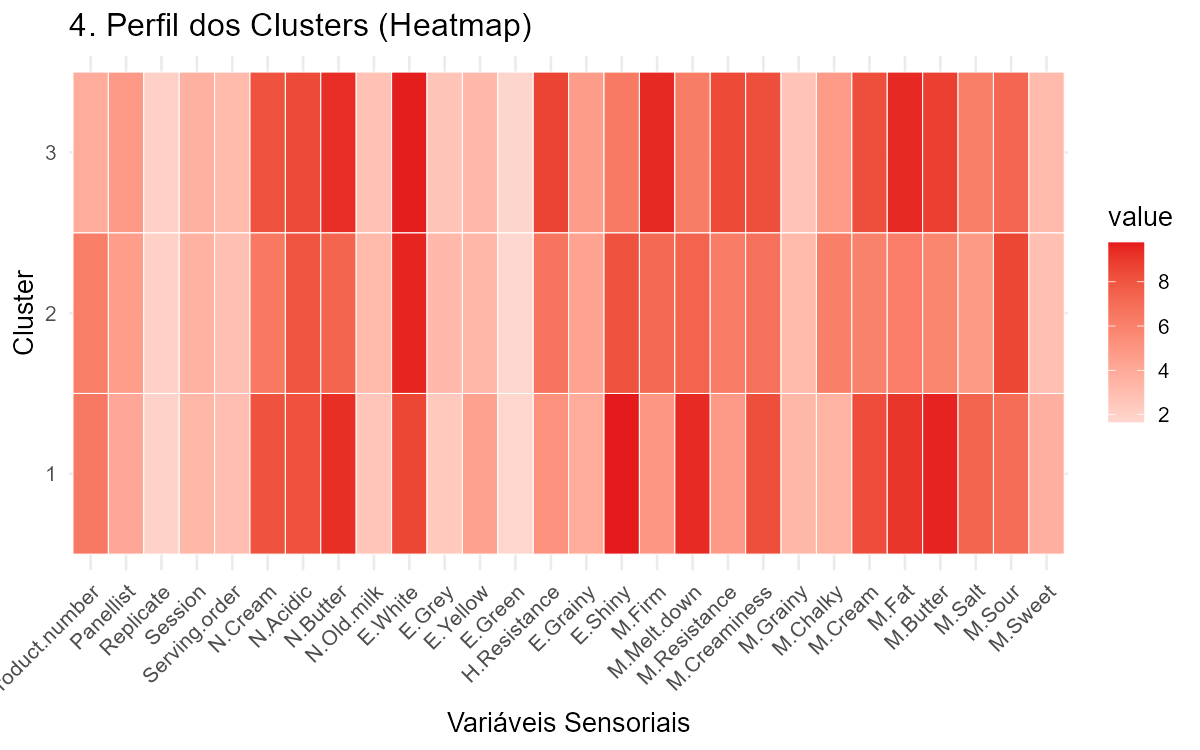
\includegraphics[width=0.92\textwidth]{fig/04_heatmap.png}
\caption{Heatmap do perfil médio de cada cluster por atributo sensorial. Tons quentes indicam valores acima da média; tons frios, abaixo --- revelando a assinatura de cada grupo.}
\end{figure}

\end{document}
